% Generated from main.typ. Typst is authoritative; regeneration overwrites this file.
\documentclass{qlnotes-export}

\title{MATH 597: Measure Theory}
\subtitle{Typst-first course notes and worked homeworks}
\author{Qiulin Fan}
\date{Winter 2025}

\begin{document}
\mainmatter
\chapter{Homework 3: on Lebesgue-Stieljes measures(30/40)}\label{homework-3-on-lebesgue-stieljes-measures3040}

\emph{None of the following questions will be graded. Do them, but do not hand them in}.

\section{Fun facts about increasing functions}\label{fun-facts-about-increasing-functions}

Let \(F:{\mathbb{R}}\rightarrow{\mathbb{R}}\) be an increasing function, that is, \(F(x) \leq F(y)\) whenever \(x \leq y\).

\begin{itemize}
\item
  Prove that the following limits exist (and make sure you understand the definitions):

  \begin{itemize}
  \item
    \(F(a - ) := \lim_{x\rightarrow a -}F(x) \in {\mathbb{R}}\) and \(F(a + ) := \lim_{x\rightarrow a +}F(x) \in {\mathbb{R}}\) for \(a \in {\mathbb{R}}\);
  \item
    \(F(\infty) := \lim_{x\rightarrow\infty}F(x) \in ( - \infty,\infty\rbrack\);
  \item
    \(F( - \infty) := \lim_{x\rightarrow - \infty}F(x) \in \lbrack - \infty,\infty)\).
  \end{itemize}
\item
  Fix any \(a \in {\mathbb{R}}\).

  \begin{itemize}
  \item
    Prove that \(F(a - ) \leq F(a) \leq F(a + )\);
  \item
    Prove that \(F\) is continuous at \(a\) iff \(F(a - ) = F(a + )\).
  \end{itemize}

  We say that a function is \emph{left continuous} if \(F(a - ) = F(a)\) for every \(a \in {\mathbb{R}}\). It is \emph{right-continuous} if instead \(F(a + ) = F(a)\) for every \(a \in {\mathbb{R}}\).
\item
  If \(X\) is a metric space (or, more generally, a topological space), then a function \(f:X\rightarrow{\mathbb{R}}\) is \emph{upper semicontinuous} if the set \(\left\{ {x \in X \mid f(x) < a} \right\}\) is open for every \(a \in {\mathbb{R}}\). It is \emph{lower semicontinuous} if instead the set \(\left\{ {x \in X \mid f(x) > a} \right\}\) is open for every \(a \in {\mathbb{R}}\). Prove that our function \(F:{\mathbb{R}}\rightarrow{\mathbb{R}}\) is right-continuous (resp. left continuous) iff it is upper semicontinuous (resp.~lower semicontinuous). Give an example showing that this is no longer true if \(F\) is not assumed increasing.
\item
  Prove that the following are equivalent:

  \begin{itemize}
  \item
    \(F\) is surjective;
  \item
    \(F\) is continuous, \(F(\infty) = \infty\), and \(F( - \infty) = - \infty\).
  \end{itemize}
\item
  Let \(A \subset {\mathbb{R}}\) be the set of points where \(F\) fails to be continuous. Prove that \(A\) is a countable (i.e. empty, finite, or countably infinite) set. \emph{Hint}: prove that for any integers \(m,n \geq 1\), the set of points \(x \in \lbrack - m,m\rbrack\) where \(F(x + ) - F(x - ) \geq 1/n\) is finite.
\end{itemize}

\section{Locally finite measures}\label{locally-finite-measures}

If \(X\) is a metric space (or, more generally, a topological space), then a Borel measure \(\mu\) on \(X\) is said to be \emph{locally finite} if \(\mu(K) < \infty\) for every compact set \(K \subset X\). Now let \(\mu\) be a Borel measure on \(\mathbb{R}\), that is \(\mu:\mathcal{B}({\mathbb{R}})\rightarrow\lbrack 0,\infty\rbrack\) satisfies \(\mu(\varnothing) = 0\) and is countably additive.

\begin{itemize}
\item
  Prove that the following are equivalent:

  \begin{itemize}
  \item
    \(\mu\) is locally finite;
  \item
    \(\mu(\lbrack - N,N\rbrack) < \infty\) for every \(N \geq 0\);
  \item
    \(\mu(I) < \infty\) for every bounded interval \(I\).
  \end{itemize}
\item
  Prove that if \(\mu\) is locally finite, then \(\mu\) is \(\sigma\)-finite. Is the converse true? Give a proof or a counterexample.
\end{itemize}

\section{Basic formulas for LS measures}\label{basic-formulas-for-ls-measures}

Let \(F:{\mathbb{R}}\rightarrow{\mathbb{R}}\) be a distribution function, and \(\mu = \mu_{F}\) the associated Lebesgue--Stieltjes measure. From its definition using h-intervals, it follows that \(\mu((a,b\rbrack) = F(b) - F(a)\) for \(- \infty < a < b < \infty\). Using this property together with basic general properties of (\(\sigma\)-finite) measures, we proved in class that \(\mu((a,b)) = F(b - ) - F(a)\) for \(\infty < a \leq b < \infty\). Using a similar strategy, prove the following:

\begin{itemize}
\item
  \(\mu(\lbrack a,b\rbrack) = F(b) - F(a - )\) for \(- \infty < a \leq b < \infty\);
\item
  \(\mu(\lbrack a,b)) = F(b - ) - F(a - )\) for \(- \infty < a \leq b < \infty\);
\item
  \(\mu(\left\{ a \right\})) = F(a) - F(a - )\) for \(- \infty < a < \infty\);
\item
  \(\mu(( - \infty,b\rbrack) = F(b) - F( - \infty)\) for \(- \infty < b < \infty\);
\item
  \(\mu(( - \infty,b)) = F(b - ) - F( - \infty)\) for \(- \infty < b < \infty\);
\item
  \(\mu((a,\infty)) = F(\infty) - F(a)\) for \(- \infty < a < \infty\);
\item
  \(\mu(\lbrack a,\infty)) = F(\infty) - F(a - )\) for \(- \infty < a < \infty\);
\item
  \(\mu(\lbrack - \infty,\infty)) = F(\infty) - F( - \infty)\).
\end{itemize}

\section{Vitali sets}\label{vitali-sets}

For \(x,y \in \lbrack - 1,1\rbrack\), write \(x \sim y\) iff \(x - y \in {\mathbb{Q}}\).

\begin{itemize}
\item
  Show that \(\sim\) is an equivalence relation, i.e. show that (i) \(x \sim x\), (ii) \(x \sim y\) implies \(y \sim x\), (iii) if \(x \sim y\) and \(y \sim z\), then \(x \sim z\).
\item
  The set \(\lbrack - 1,1\rbrack\) is partitioned into equivalence classes. Let \(V \subset \lbrack - 1,1\rbrack\) be a set containing exactly one element from each equivalence class. (Here, we use the Axiom of choice.) We call \(V\) a \emph{Vitali set}. Let \(\left\{ {r_{1},r_{2},\ldots} \right\} = \lbrack - 2,2\rbrack \cap {\mathbb{Q}}\). Define \(V_{i} = r_{i} + V = \left\{ {r_{i} + x \mid x \in V} \right\}\). Prove that the sets \(V_{1},V_{2},\ldots\) are mutually disjoint, and that

  \[\lbrack - 1,1\rbrack \subset \bigcup\limits_{i = 1}^{\infty}V_{i} \subset \lbrack - 3,3\rbrack.\]
\end{itemize}

\section{Vitali sets, season 2}\label{vitali-sets-season-2}

Let \(V \subset \lbrack - 1,1\rbrack\) be a Vitali set (see above).

\begin{itemize}
\item
  Using the translation invariance of Lebesgue measure, prove \(V\) is not Lebesgue measurable.
\item
  Prove that if \(E\) is a Lebesgue measurable set and satisfies \(E \subset V\), then \(m(E) = 0\).
\item
  Using the technique in~(a), prove the following statement: if \(A \subset {\mathbb{R}}\) is any Lebesgue measurable set with \(m(A) > 0\), then \(A\) contains a set which is not Lebesgue measurable.
\end{itemize}

\section{The middle-thirds Cantor set}\label{the-middle-thirds-cantor-set}

Let \(C\) be the middle-thirds Cantor set, defined as

\[C := \bigcap\limits_{n = 1}^{\infty}C_{n},\]

where

\[C_{n} := \bigcup\limits_{a_{1},\ldots,a_{n} \in {\{{0,2}\}}}\lbrack\sum\limits_{i = 1}^{n}\frac{a_{i}}{3^{i}},\sum\limits_{i = 1}^{n}\frac{a_{i}}{3^{i}} + \frac{1}{3^{n}}\rbrack\]

\begin{itemize}
\item
  Set \(C_{0} = \lbrack 0,1\rbrack\). Show that \(C_{n} \subset C_{n - 1}\) for all \(n \geq 1\). Also prove that \(C_{n}\) is the union of \(2^{n}\) \emph{disjoint} closed intervals, that the set \(U_{n} := C_{n - 1}\backslash C_{n}\) is the union of the middle thirds open intervals of the disjoint closed intervals of \(C_{n - 1}\), and that

  \[U_{n} = \bigcup\limits_{a_{1},\cdots,a_{n - 1} \in {\{{0,2}\}}}(\sum\limits_{i = 1}^{n - 1}\frac{a_{i}}{3^{i}} + \frac{1}{3^{n}},\sum\limits_{i = 1}^{n - 1}\frac{a_{i}}{3^{i}} + \frac{2}{3^{n}}).\]

  (We interpret this as the interval \((1/3,2/3)\) when \(n = 1\).) Thus, \(C\) is the set obtained by removing successive middle thirds of the remaining disjoint closed intervals starting with \(\lbrack 0,1\rbrack\). Sketch the first few sets \(C_{n}\) and \(U_{n}\).
\item
  Show that \(C\) is a compact set, and that \(m(C) = 0\), where \(m\) denotes Lebesgue measure. Also show that \(C\) does not contain any non-empty open interval \((a,b)\).
\item
  Show that \(C\) equals the set of numbers \(x \in \lbrack 0,1\rbrack\) which have a base-3 expansion of the form \(x = 0.a_{1}a_{2}a_{3}\cdots\) where \(a_{i}\) is either \(0\) or \(2\), i.e.~

  \[C = \left\{ {\sum\limits_{i = 1}^{\infty}\frac{a_{i}}{3^{i}} \mid \ a_{i} \in \left\{ {0,2} \right\}\ \text{for all}\ i \in {\mathbb{N}}} \right\}.\]

  (Note: A point may have two base-3 expansions such as \(1/3 = 0.1000\ldots = 0.0222\ldots\); this number is in \(C\) since one of the expansions is of the desired form.)
\item
  Show that \(\frac{1}{4},\frac{9}{13} \in C\) but \(\frac{5}{36} \notin C\).
\end{itemize}

\section{The Devil's Staircase: an increasing function build on Cantor set}\label{the-devils-staircase-an-increasing-function-build-on-cantor-set}

Let \(C\) be the middle-thirds Cantor set, and define \(F:C\rightarrow\lbrack 0,1\rbrack\) by

\[F(x) = \sum\limits_{i = 1}^{\infty}\frac{a_{i}/2}{2^{i}}\]

for \(x = \sum_{i = 1}^{\infty}\frac{a_{i}}{3^{i}}\), \(a_{i} \in \left\{ {0,2} \right\}\).

\begin{itemize}
\item
  Prove that \(F\) is an increasing function, and that \(F(C) = \lbrack 0,1\rbrack\).
\item
  Suppose that \(x,y \in C\) and \(x < y\). Prove that \(F(x) = F(y)\) iff \(x\) and \(y\) are the endpoints of a removed open interval, that is, one of the \(2^{n - 1}\) disjoint open intervals whose union equals \(U_{n} = C_{n - 1}\backslash C_{n}\) for some \(n \geq 1\).
\item
  Prove that \(F:C\rightarrow\lbrack 0,1\rbrack\) extends uniquely to a continuous function which is constant on all the intervals in \(U_{n}\), \(n \geq 1\). Sketch the graph of \(F\). \emph{Hint}: to prove continuity, it suffices to show that \(F(\lbrack 0,1\rbrack) = \lbrack 0,1\rbrack\) (Why?)
\item
  Prove that \(F'(x) = 0\) for a.e.~\(x\). In other words, there exists a set \(E \subset \lbrack 0,1\rbrack\) such that \(m(E) = 0\), and such that \(\lim_{h\rightarrow 0}(F(x + h) - F(x))/h = 0\) for \(x \in \lbrack 0,1\rbrack\backslash E\).
\end{itemize}

(Remark 1: because of~(c) and~(d), the graph of \(F\) is called the \emph{Devil's Staircase}; it is horizontal almost everywhere, and has no vertical jumps, but nevertheless climbs upwards.)

(Remark 2: the fact that \(F(C) = \lbrack 0,1\rbrack\) implies that \(C\) has the same cardinality as \(\lbrack 0,1\rbrack\), in particular the Cantor set is uncountable.)

\emph{Some of the following questions will be graded. Do them, and do hand them in}.

\section{fun facts about distribution functions}\label{fun-facts-about-distribution-functions}

\begin{itemize}
\item
  Let \(A \subset {\mathbb{R}}\) be a countable set. Exhibit a distribution function \(F\) that is discontinuous at every point in \(A\), but continuous everywhere else. Justify your answer. \emph{Hint}: play around with the Heaviside function.
\item
  Let \(F:{\mathbb{R}}\rightarrow{\mathbb{R}}\) be an increasing function. Prove that there exists a unique distribution function \(G\) such that \(G(x) = F(x)\) for all points \(x\) where \(F\) is continuous. \emph{Hint}: there is a simple formula for \(G\) in terms of \(F\).
\end{itemize}

\begin{qlsolution}{Solution}

\textbf{of (a):}\\
We list \(A = \left\{ a_{n} \right\}_{n = 1}^{\infty}\) as a sequence to label its elements. Define:

\[F(x) = \sum\limits_{n = 1}^{\infty}\frac{1}{2^{n}}H(x - a_{n})\]

where \(H(x)\) is the Heaviside function: \(H(x) = \left\{ \begin{matrix}
{0,} & {x < 0,} \\
{1,} & {x \geq 0.}
\end{matrix} \right.\).\\
\textbf{Claim 1.1 \(F\) is non-decreasing}.\\
Proof: Suppose \(y > x \in {\mathbb{R}}\), then \(H(y - a_{n}) \geq H(x - a_{n})\) for each \(n \in {\mathbb{N}}\), so we have \(F(y) \geq F(x)\).\\
\strut \\
\textbf{Claim 1.2 \(F\) is right continuous but not left continuous (thus discontinuous) at every \(a_{n}\).}\\
Proof: Let \(\epsilon > 0\).\\
We take \(N \in {\mathbb{N}}\) s.t. \(\sum_{k \geq N,n \in {\mathbb{N}}}\frac{1}{2^{k}} < \epsilon\).\\
Then we take \(\delta > 0\) such that \(a_{1},a_{2},\cdots,a_{N} \notin (a_{n},a_{n} + \delta)\).(This can be done since there are only finite points here)\\
Thus \(\forall y \in (a_{n},a_{n} + \delta)\), we have \(\left. |F(y) - F(a_{n}) \middle| < \epsilon \right.\), since \(F(y) < F(a_{n}) + \sum_{k \geq N,n \in {\mathbb{N}}}\frac{1}{2^{k}}\). Since \(\epsilon\) is arbitrary, this finishes the proof that \(F\) is right continuous at \(a_{n}\).\\
Also, \(\forall y < a_{n}\), we have \(F(y) < F(a_{n}) - \frac{1}{2^{n}}\), which means that \(\left. |F(y) - F(a_{n}) \middle| > \frac{1}{2^{n}} \right.\) for any \(y\) on the left, so \(F\) is not left continuous at \(a_{n}\).\\
\strut \\
\textbf{Claim 1.3: \(F\) is continuous at every \(x \in {\mathbb{R}}\backslash A\).}\\
Proof: This is similar to the proof in Claim 1.2.\\
Fix \(x \in {\mathbb{R}}\backslash A\). Let \(\epsilon > 0\).\\
We take \(N \in {\mathbb{N}}\) s.t. \(\sum_{k \geq N,n \in {\mathbb{N}}}\frac{1}{2^{k}} < \epsilon\).\\
Then we take \(\delta > 0\) such that \(a_{1},a_{2},\cdots,a_{N} \notin (a_{n} - \delta,a_{n} + \delta)\). This can be done since there are only finite points here.\\
Thus \(\forall y \in (a_{n} - \delta,a_{n} + \delta)\), we have \(\left. |F(y) - F(a_{n}) \middle| < \sum_{k \geq N,n \in {\mathbb{N}}}\frac{1}{2^{k}} < \epsilon \right.\).\\
\strut ~Since \(\epsilon\) is arbitrary, this finishes the proof that \(F\) is continuous at \(x\).\\
\strut \\
By claim 1.1, 1.2, 1.3, we have proved that \(F\) is a distribution function that is discontinuous at every point of \(A\) but continuous elsewhere.\\
\strut \\

\end{qlsolution}

\begin{proof}

\textbf{of (b):}\\
Given an increasing function \(F:{\mathbb{R}}\rightarrow{\mathbb{R}}\), we define \(G:{\mathbb{R}}\rightarrow{\mathbb{R}}\) by:

\[G(x) = \lim\limits_{y\rightarrow x^{+}}F(y).\]

We will show that this is the unique distribution function \(G\) such that \(G(x) = F(x)\) for all points \(x\) where \(F\) is continuous.\\
\textbf{Incresing:} Since \(F\) is increasing, for any \(x < y\) we have \(F(x) \leq F(y)\). Thus, for any \(x < y\) we have:

\[G(x) = \lim\limits_{z\rightarrow x^{+}}F(z) \leq \lim\limits_{z\rightarrow y^{+}}F(z) = G(y).\]

Thus, \(G\) is increasing.\\
\textbf{Right-continuity:} Since \(F\) is an increasing function, it can only have jump discontinuities, and the right limit exists for all \(X\). By construction, \(G\) is right-ctn.\\
Above finishes the proof that \(G\) is a distribution function.\\
\textbf{Agree with \(F\) at ctn point:} \(G(x) = F(x)\) where \(F\) is continuous at \(x\), since \(G(x) = \lim_{y\rightarrow x^{+}}F(y) = F(x)\) there.\\
It remains to show that it is unique.\\
Suppose \(R\) is another such function. It suffices to show: \(R\) agrees with \(G\) on discontinuous points of \(F\).\\
Since \(R,G\) are right continuous, their right limit must exist at each point. Therefore, let \(x\) be an arbitrary point where \(F\) is discontinuous at \(x\), \textbf{it suffices to show that there is a sequence \(\left\{ x_{n} \right\}\) approaching \(x\), such that \(\lim_{n}G(x_{n}) = \lim_{n}R(x_{n})\).}\\
Since \(F\) is increasing, the points where \(F\) is disctn is at most countable. Therefore \textbf{the points where \(F\) is ctn, denote it as \(C\), is dense in \(\mathbb{R}\).} Thus we can pick a sequence \(\left\{ x_{n} \right\}\) in \(C\) approaching \(x\), then \(G(x_{n}) = R(x_{n}) = F(x_{n})\) for each \(n\), impling that \(\lim_{n}G(x_{n}) = \lim_{n}R(x_{n})\). This finishes the proof of uniqueness.

\end{proof}

\section{Finding intervals}\label{finding-intervals}

Let \(E \subset {\mathbb{R}}\) be a Lebesgue measurable subset with \(m(E) > 0\). Prove that for every \(\alpha \in (0,1)\) there exists an (nonempty) bounded open interval \(I\) such that \(m(E \cap I) \geq \alpha m(I)\). \emph{Hint}: first reduce to the case when \(E\) is bounded, then use outer regularity.

\begin{proof}

Let \(\alpha \in (0,1)\) be arbitrary and fix it.\\
We first consider the case that \(E\) is bounded. By outer regularity of Lebesgue measure, there exists an open set \(G\) such that

\[E \subset G\quad\text{and}\quad m(G) - m(E) \leq (1/\alpha - 1) m(E)\]

since \(\alpha \in (0,1)\). Then we have:

\[m(G) \leq 1/\alpha m(E)\]

Note that in \(\mathbb{R}\), an open set is just a countable disjoint union of open intervals. We write:

\[G = \bigsqcup\limits_{i \in {\mathbb{N}}}I_{i}\]

Since \(E \subset G\), we have:

\[E = \bigsqcup\limits_{i \in {\mathbb{N}}}(I_{i} \cap E)\]

Thus

\[m(E) = \sum\limits_{i \in {\mathbb{N}}}m(I_{i} \cap E) \geq \alpha\sum\limits_{i \in {\mathbb{N}}}m(I_{i})\]

So \textbf{there must exist some \(i\) such that \(m(I_{i} \cap E) \geq \alpha\, m(I_{i})\), otherwise contradicting with the ineq above.}\\
This finishes the proof of the bounded case.\\
The we consider the case when \(E\) is unbounded. We can write

\[E = \bigsqcup\limits_{n \in {\mathbb{Z}}}(E \cap (n,n + 1\rbrack)\]

where each \(E_{n} := E \cap (n,n + 1\rbrack\) is bounded.\\
We apply the case where \(E\) is bounded, confirming that there is some interval \(I\) such that \(m(E_{1} \cap I) \geq \alpha m(I)\). By monotonicity of measure, we have \(m(E \cap I) \geq m(E_{1} \cap I) \geq \alpha m(I)\).

\end{proof}

\section{So many differences}\label{so-many-differences}

Let \(E \subset {\mathbb{R}}\) be a Lebesgue measurable subset with \(m(E) > 0\).

\begin{itemize}
\item
  Prove that the set

  \[E - E := \left\{ {x - y \mid x,y \in E} \right\} \subset {\mathbb{R}}\]

  contains a nonempty open interval centered at the origin. \emph{Hint}: use the previous exercise with \(\alpha\) large enough, together with the translation invariance of Lebesgue measure.
\item
  Prove that there exists \(\epsilon > 0\) such that \(E \times E \subset {\mathbb{R}}^{2}\) intersects every line \(y = x + t\) with \(\left. |t \middle| < \epsilon \right.\).
\item
  Let \(C \subset {\mathbb{R}}\) be the middle-third Cantor set (so \(m(C) = 0\)). Does \(C - C\) contain a nonempty open interval centered at the origin?
\end{itemize}

\begin{proof}

\textbf{of (a):}

\begin{center}

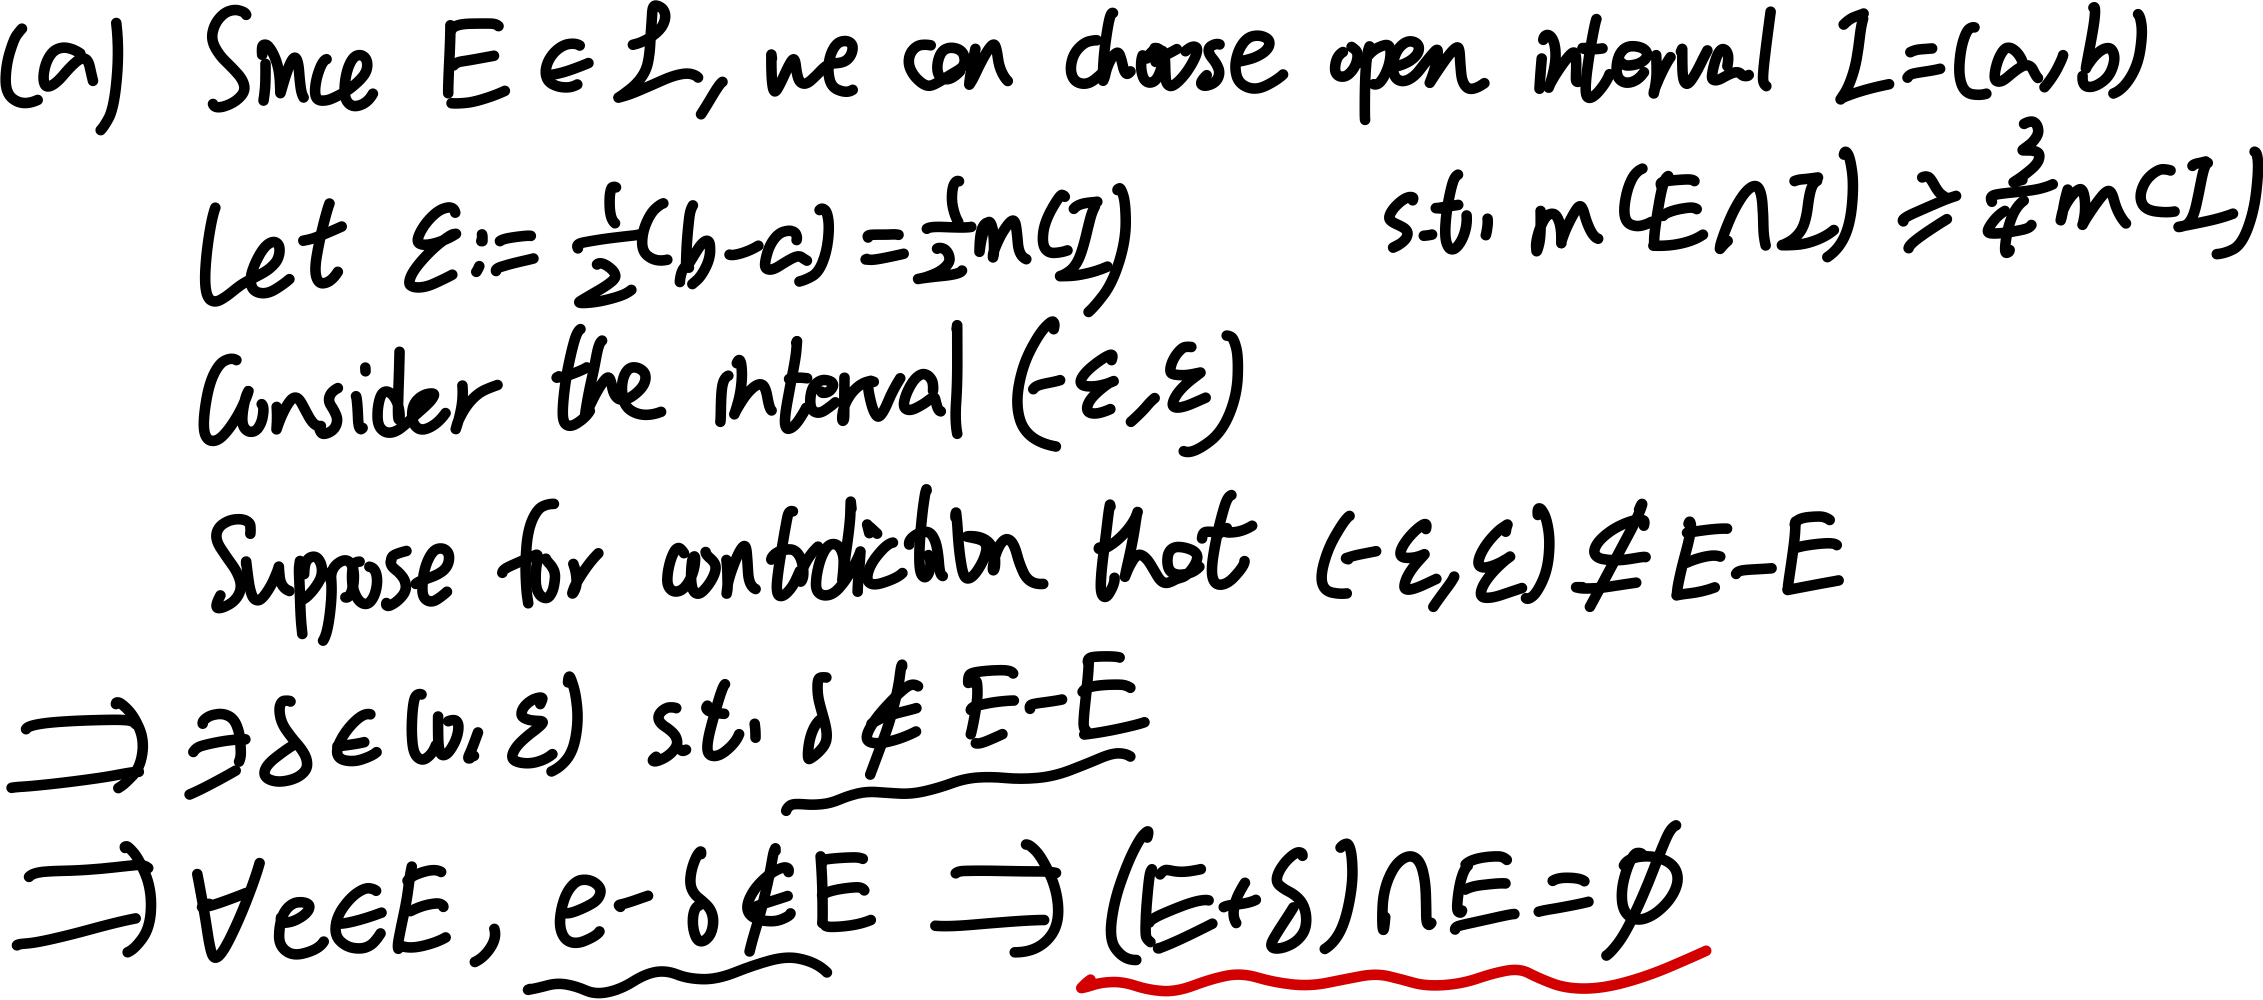
\includegraphics[width=0.65\linewidth,height=\textheight,keepaspectratio]{assets/main--figure-raster-009.png}

\end{center}

\begin{center}

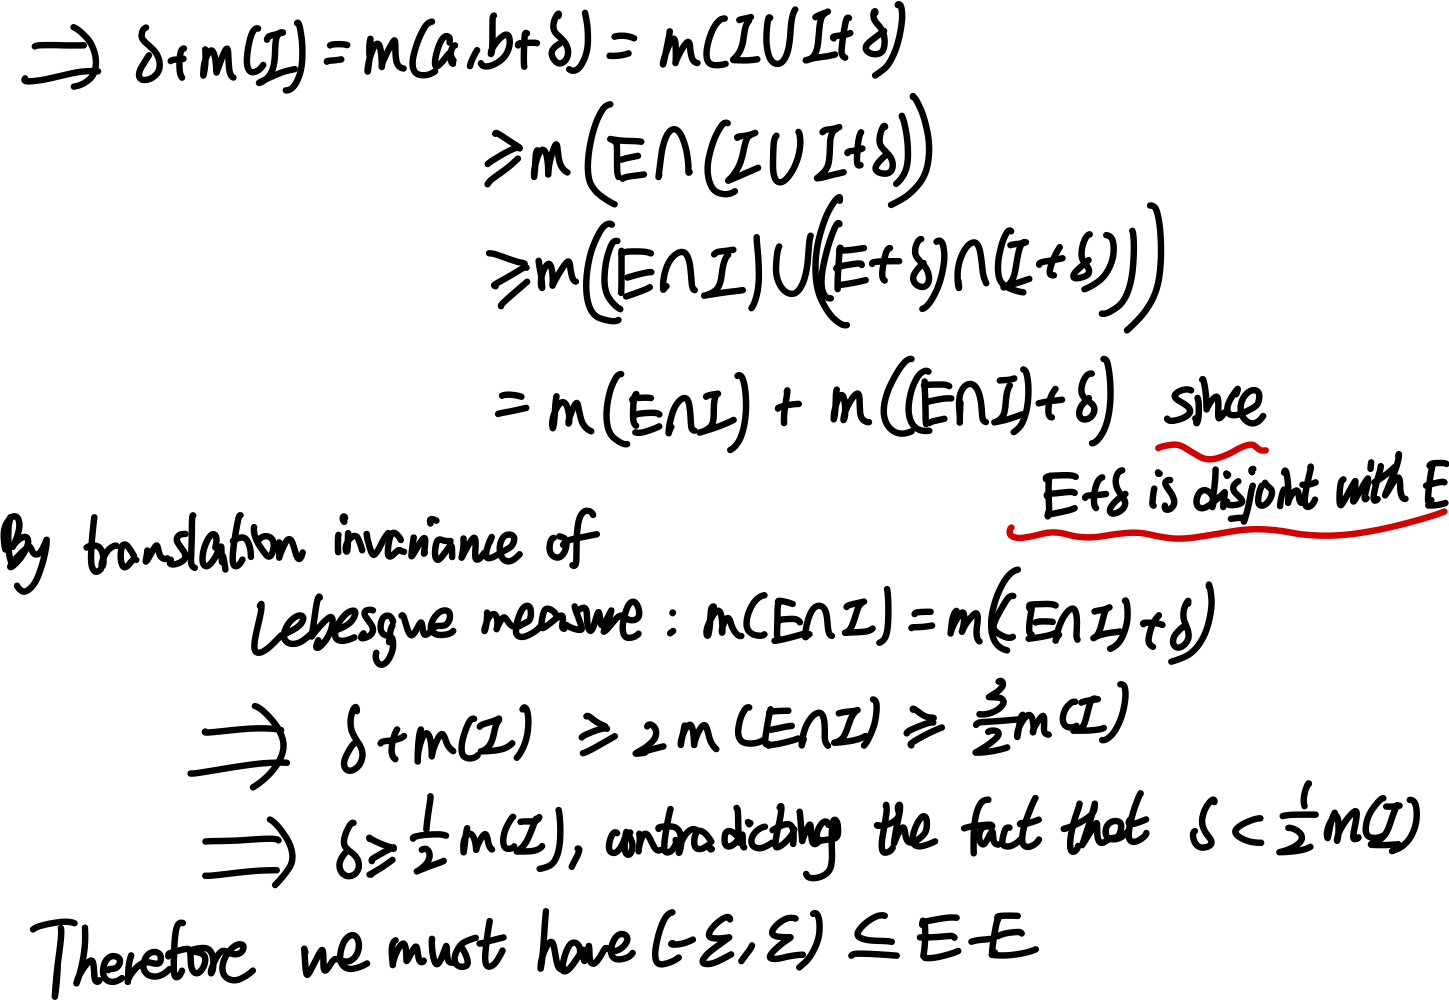
\includegraphics[width=0.7\linewidth,height=\textheight,keepaspectratio]{assets/main--figure-raster-010.png}

\end{center}

\end{proof}

\begin{proof}

\textbf{of (b):}\\
Consider taking \(\epsilon\) as the one in (a) where the interval contained in \(E - E\) is \(( - \epsilon,\epsilon)\), then the box \(( - \epsilon,\epsilon) \times ( - \epsilon,\epsilon)\) is contained in \(E \times E\). It trivially follows that \(E \times E \subset {\mathbb{R}}^{2}\) intersects every line \(y = x + t\) with \(\left. |t \middle| < \epsilon \right.\), since the intercept of this line with \(y\)-axis is below \(\epsilon\) and above \(- \epsilon\).

\begin{center}

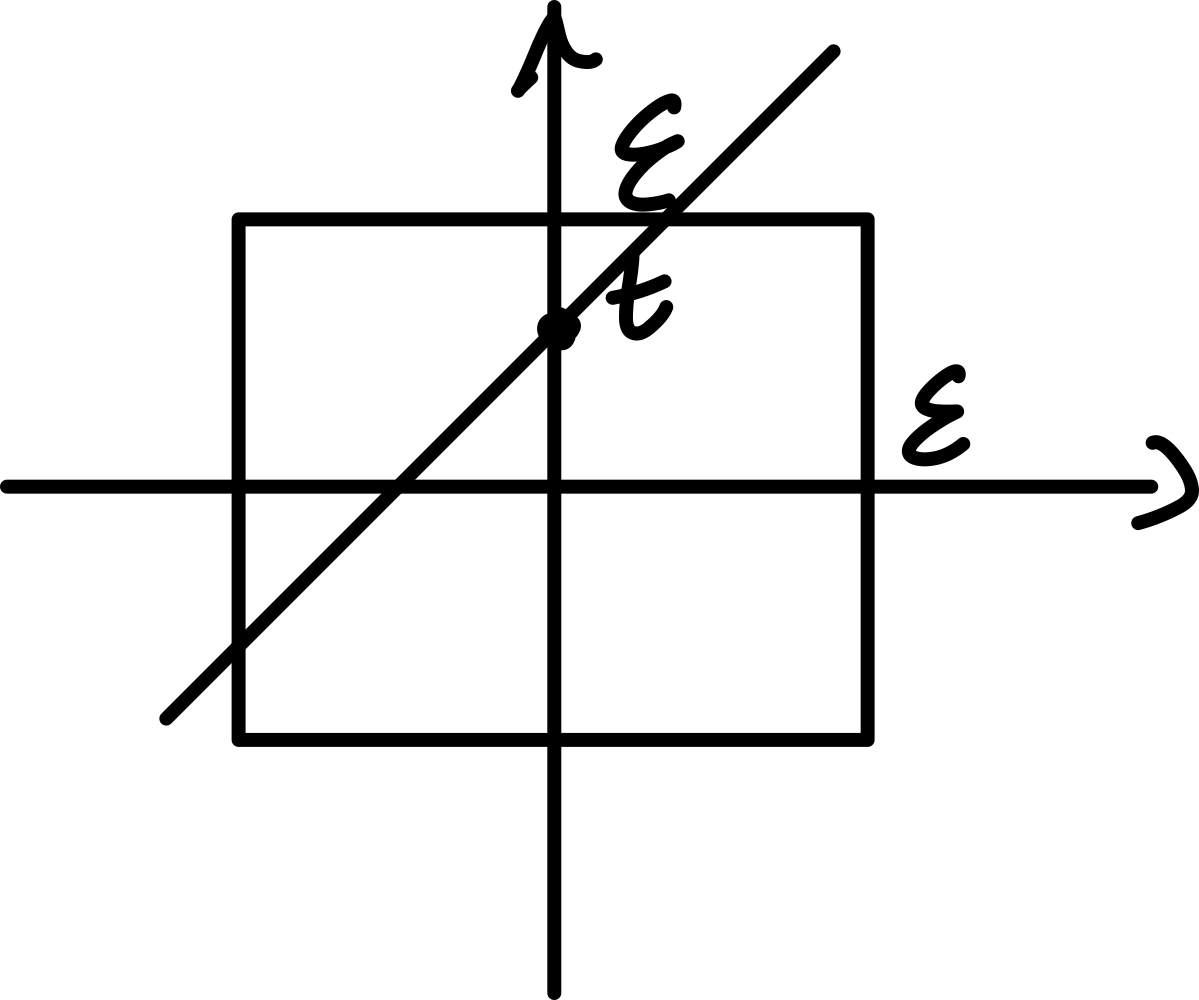
\includegraphics[width=0.25\linewidth,height=\textheight,keepaspectratio]{assets/main--figure-raster-011.png}

\end{center}

\end{proof}

\begin{qlsolution}{Solution}

\textbf{of (c):} \(C - C\) contain a nonempty open interval centered at the origin, and we will prove that one such interval is \(( - 1,1)\).

\begin{proof}

Recall the balanced ternary representation of \(\lbrack - 1/2,1/2\rbrack\): \(\forall x \in \lbrack - 1/2,1/2\rbrack\), there is a seq of \((a_{n})_{n \in {\mathbb{N}}}\) in \(\left\{ {- 1,0,1} \right\}\) s,t,

\[x = \sum\limits_{n = 1}^{\infty}\frac{a_{n}}{3^{n}},\qquad a_{n} \in \left\{ {- 1,0,1} \right\},\]

Thus every \(x \in \lbrack - 1,1\rbrack\) can be halved, ternary expanded and then doubled to recover:

\[\begin{matrix}
{x = 2\sum\limits_{n = 1}^{\infty}\frac{a_{n}}{3^{n}}} & {= \sum\limits_{n = 1}^{\infty}\frac{2a_{n}}{3^{n}},\qquad a_{n} \in \left\{ {- 1,0,1} \right\}} \\
 & {= \sum\limits_{n = 1}^{\infty}\frac{b_{n}}{3^{n}},\qquad b_{n} \in \left\{ {- 2,0,2} \right\}}
\end{matrix}\]

And by the problem "The middle-thirds Cantor set", we learned that

\[C = \left\{ {\sum\limits_{i = 1}^{\infty}\frac{a_{i}}{3^{i}} \mid \ a_{i} \in \left\{ {0,2} \right\}\ \text{for all}\ i \in {\mathbb{N}}} \right\}.\]

Therefore we can write every number \(x \in \lbrack - 1,1\rbrack\) into a difference of two \(x,y \in C\), i.e. an element of \(C - C\):

\[\begin{matrix}
x & {= \sum\limits_{n = 1}^{\infty}\frac{b_{n}}{3^{n}},\qquad b_{n} \in \left\{ {- 2,0,2} \right\}} \\
 & {= \sum\limits_{n = 1}^{\infty}\frac{p_{n} - q_{n}}{3^{n}},\qquad p_{n},q_{n} \in \left\{ {- 2,0,2} \right\}} \\
 & {= \sum\limits_{n = 1}^{\infty}\frac{p_{n}}{3^{n}} - \sum\limits_{n = 1}^{\infty}\frac{q_{n}}{3^{n}},\qquad p_{n},q_{n} \in \left\{ {- 2,0,2} \right\}}
\end{matrix}\]

since each series converges independently. Here we let \(p_{n} = 2,q_{n} = 0\) if \(b_{n} = 2\); \(p_{n} = 0,q_{n} = 2\) if \(b_{n} = - 2\), \(p_{n} = 0,q_{n} = 0\) if \(b_{n} = 0\).\\
Thus \(x \in C - C\), so \(\lbrack - 1,1\rbrack \subset C - C\).

\end{proof}

\end{qlsolution}

\section{a holey set}\label{a-holey-set}

Let \((x_{n})_{1}^{\infty}\) be a countable dense sequence in \((0,1)\). For each \(t > 0\), consider the set

\[A_{t} := \lbrack 0,1\rbrack\backslash\bigcup\limits_{n = 1}^{\infty}(x_{n} - 2^{- n}t,x_{n} + 2^{- n}t).\]

\begin{itemize}
\item
  Prove that \(A_{t}\) is a compact (possibly empty) subset of \(\mathbb{R}\). Also prove that \(A_{t}\) has empty interior, that is, \(A_{t}\) contains no nonempty open set.
\item
  Prove that \(t\mapsto m(A_{t})\) is continuous.
\item
  Prove that there exists \(t > 0\) such that \(m(A_{t}) = 597/2025\).
\end{itemize}

\begin{proof}

\textbf{of a:}

\begin{center}

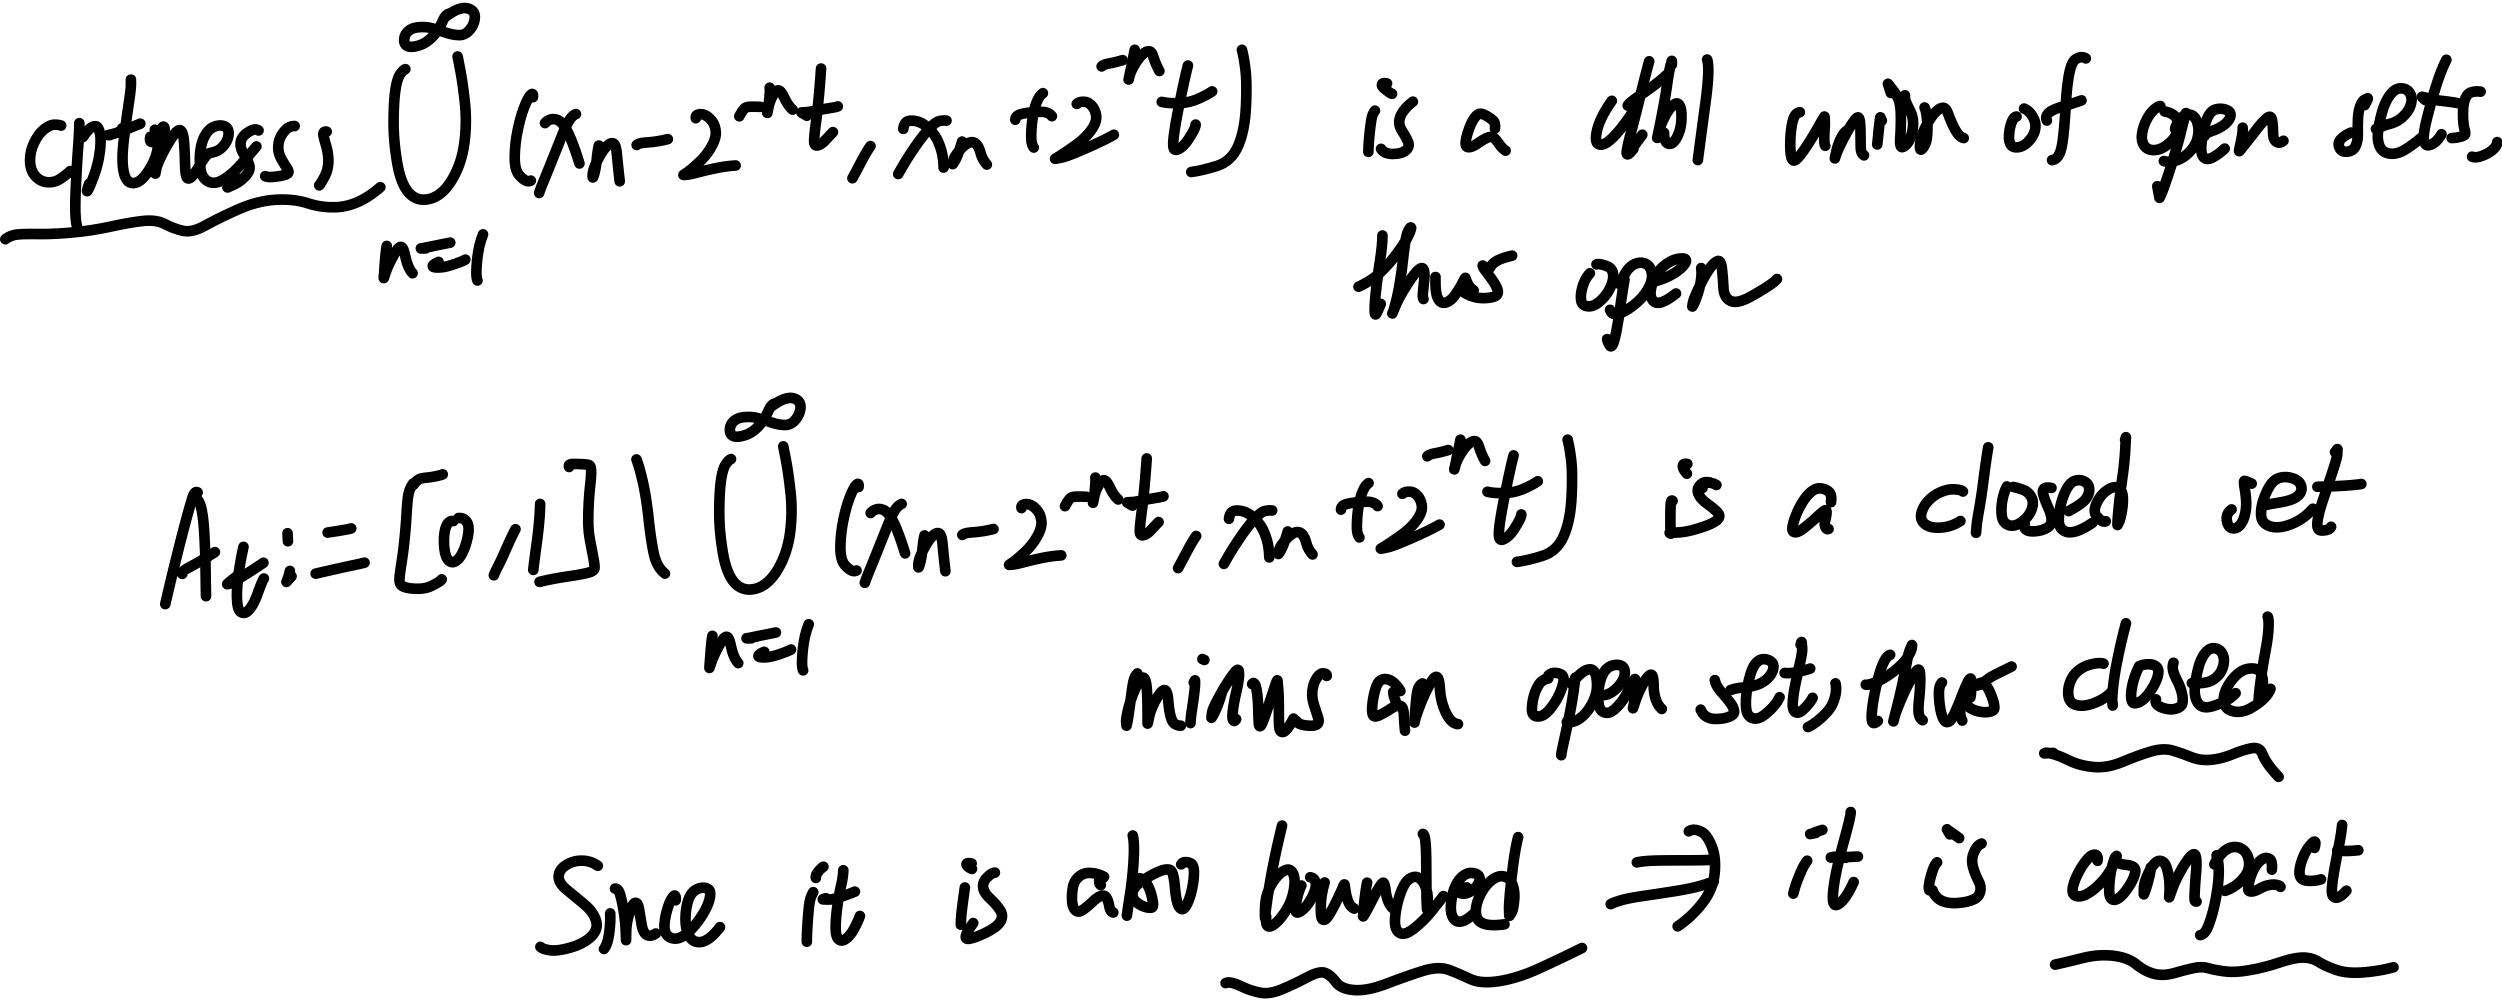
\includegraphics[width=0.7\linewidth,height=\textheight,keepaspectratio]{assets/main--figure-raster-012.png}

\end{center}

\end{proof}

\begin{proof}

\textbf{of b:} Define for each \(n \in {\mathbb{N}}\)

\[I_{n}(t) = (x_{n} - 2^{- n}t,x_{n} + 2^{- n}t)\]

Then

\[A_{t} = \lbrack 0,1\rbrack\backslash\bigcup\limits_{n = 1}^{\infty}I_{n}(t)\]

So

\[m(A_{t}) = m(\lbrack 0,1\rbrack) - m(\bigcup\limits_{n = 1}^{\infty}I_{n}(t)) = 1 - m(\bigcup\limits_{n = 1}^{\infty}I_{n}(t))\]

\textbf{Thus it suffices to show \(t\mapsto m(\bigcup_{n = 1}^{\infty}I_{n}(t))\) is continuous.}

Let \(\epsilon > 0\). Let \(t > 0\).\\
We consider \(p \in (t,t + \epsilon/2)\):

By set inclusion relation and measure's property, we have:

\[m(\bigcup\limits_{n = 1}^{\infty}I_{n}(p)) - m(\bigcup\limits_{n = 1}^{\infty}I_{n}(t)) = m(\bigcup\limits_{n = 1}^{\infty}I_{n}(p)\backslash\bigcup\limits_{n = 1}^{\infty}I_{n}(t))\]

Since

\[(\bigcup\limits_{n = 1}^{\infty}I_{n}(p))\backslash(\bigcup\limits_{n = 1}^{\infty}I_{n}(t)) \subset \bigcup\limits_{n = 1}^{\infty}(I_{n}(p)\backslash I_{n}(t))\]

We have:

\[\begin{matrix}
{m(\bigcup\limits_{n = 1}^{\infty}I_{n}(p)) - m(\bigcup\limits_{n = 1}^{\infty}I_{n}(t))} & {\leq m(\bigcup\limits_{n = 1}^{\infty}(I_{n}(p)\backslash I_{n}(t)))} \\
 & {\leq \sum\limits_{n = 1}^{\infty}(m(I_{n}(p)) - m(I_{n}(t)))} \\
 & {= \sum\limits_{n = 1}^{\infty}2 \cdot 2^{- n}(p - t)} \\
 & {= 2(p - t)} \\
 & {\leq \epsilon}
\end{matrix}\]

Similarly for \(p \in (t - \epsilon/2,t)\), we get the same bound. This finishes the proof pf (b).

\end{proof}

\begin{proof}

\textbf{of c:\\
}{ }We use the same notation of \(I_{n}(t)\) as in (b). We have:

\[m(\bigcup\limits_{n = 1}^{\infty}I_{n}(t)) \leq \sum\limits_{n = 1}^{\infty}m(I_{n}(t)) = \sum\limits_{n = 1}^{\infty}m(I_{n}(t)) = \sum\limits_{n = 1}^{\infty}2 \cdot 2^{- n}t = 2t.\]

So by choosing \(t := 1/6\), we have \(m(A_{t}) = 1 - m(\bigcup_{n = 1}^{\infty}I_{n}(t)) \geq 2/3\). And by choosing \(t := 4\), \(I_{1}(t)\) covers an interval of length \(4\), so \(A_{t} = \varnothing\), \(m(A_{t}) = 0\). By intermediate value theorem, there exists some \(t \in (1/6,4)\) such that \(m(A_{t}) = 597/2025\).

\end{proof}

\section{a Cantor measure}\label{a-cantor-measure}

(A Cantor measure.) Let \(E \subset {\mathbb{R}}\) be a nonempty compact set with the following property: for every \(x \in E\) and every \(\epsilon > 0\), the set \((x - \epsilon,x) \cup (x,x + \epsilon)\) has nonempty intersection with both \(E\) and \(E^{c}\). Prove that there exists a Borel measure \(\mu\) on \(\mathbb{R}\) with the following properties:

\begin{itemize}
\item
  if \(I \subset {\mathbb{R}}\) is a nonempty open interval, then \(\mu(I) > 0\) iff \(I \cap E \neq \varnothing\).
\item
  \(\mu(\left\{ x \right\}) = 0\) for all \(x \in {\mathbb{R}}\);
\item
  \(\mu({\mathbb{R}}) = 0.597597597\ldots\).
\end{itemize}

\emph{Hint}: set \(\mu = \mu_{F}\), where \(F\) is a distribution function whose graph is similar to the Devil's staircase above.

\begin{proof}

Write \(T := 0.597597597\ldots\)\\
Since \(E\) is compact, \(E^{c}\) is open. Also, since \(E\) is compact, it takes min and max element.\\
Thus we consider \(A := E^{c} \cap (\min E,\max E)\), this is an open set. We know any open set in \(\mathbb{R}\) is a countable disjoint union of open intervals, so \(A := E^{c} \cap (\min E,\max E) = \bigsqcup_{n = 1}^{\infty}I_{n}\) for some disjoint intervals \(I_{1} = (a_{1},b_{1}),I_{2} = (a_{2},b_{2}),\cdots\) .\\
\strut \\
Now we construct a function \(G:A\rightarrow\lbrack 0,T)\) by sending \(G(x) = \sum_{b_{i} \leq a_{N}}\frac{T}{2^{n}}\), for \(x \in I_{N}\).\\
This is an \textbf{increasing step function} since, each \(I_{n}\) is disjoint and on a fixed interval \(I_{N}\), the number of \(b_{i}\) that its \(a_{N}\) surpasses is constant. And suppose \(y > x\) is on \(I_{M}\), we have must \(G(y) \geq G(x)\) because he number of \(b_{i}\) that \(a_{M}\) surpasses is at least at many as that \(a_{N}\) surpasses.\\
And for each \(x \in A\), we have \textbf{\(G(x) < T\)}, by geometric series\\
Then we construct \(F\) out of \(G\), define:

\[\begin{matrix}
{F := \{ 0,\quad\quad x \leq \min E} \\
{\inf\left\{ {G(y) \mid y \geq x,y \in A} \right\},\quad\quad x \in (\min E,\max E)} \\
{T,\quad\quad x \geq \max E}
\end{matrix}\]

\textbf{\(F\) is increasing:} It is constant on \(( - \infty,\min E) \cup (\max E,\infty)\) and is the infimum of \(G(y)\) with \(y \geq x\) on \((\min E,\max E)\). Since \(G\) is increasing, \(F\) is also increasing.\\
\textbf{\(F\) is right continuous:} It suffices to prove the right-continuity of \(F\) on \(x \in E^{c} \cap (\min E,\max E)\).\\
Fix \(x_{0} \in E^{c} \cap (\min E,\max E)\).\\
Let \(\epsilon > 0\).\\
Let \(k \in {\mathbb{N}}\) such that \(\epsilon > \frac{T}{2^{k} + 1}\).\\
We define for each \(y\), \(S_{y} := \left\{ {b_{i} \mid x_{0} \leq b_{i} \leq y} \right\}\) as the set of all \(b_{i}\) (right endpoint of \(I_{k}\)) that is witin \(x_{0}\) and \(y\). Note that \(I_{z} \subset I_{y}\) for all \(y > z\).\\
Consider \(y_{1} := \min(\left\{ {b_{1},\cdots,b_{k}} \right\}\backslash S_{x})\).\\
Then for all \(y \in (x_{0},y_{1})\), we have:

\[F(y) \leq F(x_{0}) + \sum\limits_{i = k}^{\infty}\frac{T}{2^{i}} \leq F(x_{0}) + \epsilon\]

By defining \(\delta: = y_{1} - x_{0}\), we have shown the right continuity of \(F\).\\
(By dual reason, we can prove that \(F\) is left continuous. So \(F\) is actually continuous.) Above, we have shown that \(F\) is a distribution function.\\
\strut \\
Now let \(\mu_{F}\) be the Lebesgue-Stieljes measure associated with \(F\). We will prove for the three properties above:\\

\begin{itemize}
\item
  Let \(\left\{ x \right\}\) be a singleton set in \(\mathbb{R}\), for each \(n \in {\mathbb{N}}\), we can construct an h-intervals seq of covering of \(\left\{ x \right\}\) by \((x - 1/n,x\rbrack\) as the first covering set and \(\varnothing\) as all other covering sets.\\
  Then by the definition of \(\mu_{F}\), we have:

  \[\mu_{F}(\left\{ x \right\}) = \inf\limits_{n \in {\mathbb{N}}}(F(x) - F(x - 1/n))\]

  By continuity, it shows that \(\mu_{F}(\left\{ x \right\}) = 0\).
\item
  \[\mu_{F}({\mathbb{R}}) = \lim\limits_{x\rightarrow\infty}F(x) - \lim\limits_{x\rightarrow - \infty}F(x) = T - 0 = T = 0.597597597\cdots\]
\item
  Let \(I = (a,b)\) be a nonempty open interval.\\
  Suppose \(\mu(I) > 0\), then \(F(b) - F(a) > 0\), so by definition of \(G\), some must be at least two different intervals \(I_{n_{1}}\), \(I_{n_{2}}\) in \(A\) such that for some \(x,y \in (a,b)\), \(x \in I_{n_{1}}\) and \(y \in I_{n_{2}}\), thus \(\exists\) some \(e \in E\) such that \(e \in (x,y)\). Thus \(I \cap E \neq \varnothing\).\\
  Suppose \(I \cap E \neq \varnothing\). Let \(e \in E \cap I\). Since \(\forall\epsilon > 0\), \((x - \epsilon,x) \cup (x,x + \epsilon)\) has nonempty intersection with both \(E\) and \(E^{c}\), \(e\) has some open neighborhood \(B_{\epsilon}(e) \subset I\), intersecting two different \(I_{N}\), \(I_{M} \subset A\). Take \(n \in I_{N}\), \(m \in I_{m}\). Then \(F(m) - F(n) = G(m) - G(n) > 0\), so \(\mu_{F}(E) \geq F(m) - F(n) > 0\) by monotinicity of measure.\\
  This finishes the proof.
\end{itemize}

\end{proof}

`
\end{document}
